% ============================================================
%  DNS / DNSS con Filtro de Kalman — tau Adaptativo
%  Documentacion tecnica — Proyecto KJM
%  Compilar: xelatex -shell-escape DNS_DNSS_KalmanFilter.tex  (x2)
% ============================================================
\documentclass[12pt, a4paper]{article}

% ── Fuentes (XeLaTeX) ────────────────────────────────────────
\usepackage{fontspec}
\setmainfont{Latin Modern Roman}
\setsansfont{Latin Modern Sans}
\setmonofont[Scale=0.88]{Latin Modern Mono}
\usepackage{microtype}

% ── Geometria ────────────────────────────────────────────────
\usepackage[
  top=2.5cm, bottom=2.8cm,
  left=2.8cm, right=2.8cm,
  headheight=24.1pt
]{geometry}

% ── Colores ──────────────────────────────────────────────────
\usepackage[dvipsnames, table]{xcolor}
\definecolor{azulprincipal}{HTML}{1A3A5C}
\definecolor{azulmedio}{HTML}{2E6DA4}
\definecolor{azulclaro}{HTML}{D6E8F7}
\definecolor{azulmuyclaro}{HTML}{EEF5FC}
\definecolor{verdecod}{HTML}{1B6B3A}
\definecolor{grisclaro}{HTML}{F4F4F4}
\definecolor{grismedio}{HTML}{CCCCCC}
\definecolor{rojoacento}{HTML}{C0392B}
\definecolor{naranjacita}{HTML}{D35400}
\definecolor{verdetip}{HTML}{1E8449}
\definecolor{morado}{HTML}{6C3483}

% ── Matematicas ──────────────────────────────────────────────
\usepackage{amsmath, amssymb, amsthm, mathtools}
\usepackage{bm}

% ── Tablas ───────────────────────────────────────────────────
\usepackage{booktabs}
\usepackage{tabularx}
\usepackage{multirow}
\usepackage{array}
\usepackage{longtable}
\newcolumntype{L}[1]{>{\raggedright\arraybackslash}p{#1}}
\newcolumntype{C}[1]{>{\centering\arraybackslash}p{#1}}
\newcolumntype{R}[1]{>{\raggedleft\arraybackslash}p{#1}}

% ── TikZ ─────────────────────────────────────────────────────
\usepackage{tikz}
\usepackage{pgfplots}
\pgfplotsset{compat=1.18}
\usetikzlibrary{arrows.meta, shapes.geometric, positioning,
                fit, backgrounds, decorations.pathreplacing,
                calc, patterns}

% ── Codigo fuente ────────────────────────────────────────────
\usepackage[most]{tcolorbox}
\tcbuselibrary{listings, breakable, skins}

\lstset{
  language=Python,
  basicstyle=\small\ttfamily,
  keywordstyle=\color{azulmedio}\bfseries,
  stringstyle=\color{rojoacento},
  commentstyle=\color{verdecod}\itshape,
  numberstyle=\tiny\color{gray},
  numbers=left,
  numbersep=8pt,
  breaklines=true,
  backgroundcolor=\color{grisclaro},
  showstringspaces=false,
  tabsize=4,
  frame=none,
  xleftmargin=14pt,
  framexleftmargin=14pt,
  aboveskip=4pt,
  belowskip=4pt,
  morekeywords={True,False,None,np,pd,plt,def,return,
                import,from,as,for,in,if,elif,else},
}

% Cajas
\newtcolorbox{teoremabox}[2][]{
  enhanced, breakable,
  colback=azulmuyclaro, colframe=azulmedio,
  colbacktitle=azulprincipal, coltitle=white,
  fonttitle=\bfseries\small,
  title={#2}, sharp corners=south,
  left=6pt, right=6pt, top=4pt, bottom=4pt, #1
}
\newtcolorbox{notabox}[1][Nota]{
  enhanced, breakable,
  colback=grisclaro, colframe=grismedio,
  colbacktitle=grismedio, coltitle=black,
  fonttitle=\bfseries\footnotesize,
  title={#1}, left=6pt, right=6pt, top=3pt, bottom=3pt,
  sharp corners,
}
\newtcolorbox{tipbox}[1][Recomendacion]{
  enhanced, breakable,
  colback=white, colframe=verdetip,
  borderline west={3pt}{0pt}{verdetip},
  fonttitle=\bfseries\footnotesize,
  title={#1}, left=8pt, right=6pt, top=3pt, bottom=3pt,
  sharp corners, boxrule=0.4pt,
}
\newtcolorbox{atencionbox}[1][Atencion]{
  enhanced, breakable,
  colback=white, colframe=rojoacento,
  borderline west={3pt}{0pt}{rojoacento},
  fonttitle=\bfseries\footnotesize,
  title={#1}, left=8pt, right=6pt, top=3pt, bottom=3pt,
  sharp corners, boxrule=0.4pt,
}
\newtcblisting{codigocaja}[2][]{
  enhanced, breakable,
  colback=grisclaro, colframe=azulmedio,
  colbacktitle=azulmedio!85!black, coltitle=white,
  fonttitle=\ttfamily\small, title={#2},
  listing only,
  listing options={
    language=Python,
    basicstyle=\small\ttfamily,
    keywordstyle=\color{azulmedio}\bfseries,
    stringstyle=\color{rojoacento},
    commentstyle=\color{verdecod}\itshape,
    numberstyle=\tiny\color{gray},
    numbers=left, numbersep=6pt,
    breaklines=true, showstringspaces=false, tabsize=4,
    morekeywords={True,False,None,np,pd,plt,def,return,
                  import,from,as,for,in,if,elif,else},
  },
  left=2pt, right=2pt, top=2pt, bottom=2pt, #1
}

% ── Encabezados ──────────────────────────────────────────────
\usepackage{fancyhdr}
\pagestyle{fancy}
\fancyhf{}
\fancyhead[L]{\small\color{azulmedio}%
  \textit{DNS/DNSS Kalman Filter Adaptativo}}
\fancyhead[R]{\small\color{azulmedio}\textit{Proyecto KJM}}
\fancyfoot[C]{\small\color{grismedio}\thepage}
\renewcommand{\headrulewidth}{0.4pt}
\renewcommand{\headrule}{%
  \hbox to\headwidth{%
    \color{azulmedio}\leaders\hrule height\headrulewidth\hfill}}

% ── Hipervinculos ────────────────────────────────────────────
\usepackage[
  colorlinks=true, linkcolor=azulmedio,
  citecolor=naranjacita, urlcolor=azulmedio,
  bookmarks=true, bookmarksnumbered=true,
]{hyperref}

% ── Secciones ────────────────────────────────────────────────
\usepackage{titlesec}
\titleformat{\section}
  {\Large\bfseries\color{azulprincipal}}
  {\thesection.}{0.8em}{}
  [\color{azulmedio}\rule{\textwidth}{0.6pt}\vspace{2pt}]
\titleformat{\subsection}
  {\large\bfseries\color{azulmedio}}
  {\thesubsection.}{0.7em}{}
\titleformat{\subsubsection}
  {\normalsize\bfseries\color{azulprincipal!70!black}}
  {\thesubsubsection.}{0.6em}{}

% ── Entornos ─────────────────────────────────────────────────
\theoremstyle{plain}
\newtheorem{proposicion}{Proposicion}[section]
\theoremstyle{definition}
\newtheorem{definicion}{Definicion}[section]
\newtheorem{algoritmo}{Algoritmo}[section]
\theoremstyle{remark}
\newtheorem{observacion}{Observacion}[section]

% ── Macros matematicos ───────────────────────────────────────
\newcommand{\bbet}{\bm{\beta}}
\newcommand{\btau}{\bm{\tau}}
\newcommand{\bmu}{\bm{\mu}}
\newcommand{\beps}{\bm{\varepsilon}}
\newcommand{\bY}{\mathbf{Y}}
\newcommand{\by}{\mathbf{y}}
\newcommand{\bH}{\mathbf{H}}
\newcommand{\bF}{\mathbf{F}}
\newcommand{\bQ}{\mathbf{Q}}
\newcommand{\bR}{\mathbf{R}}
\newcommand{\bI}{\mathbf{I}}
\newcommand{\bP}{\mathbf{P}}
\newcommand{\bK}{\mathbf{K}}
\newcommand{\bG}{\mathbf{G}}
\newcommand{\bS}{\mathbf{S}}
\newcommand{\bL}{\mathbf{L}}
\newcommand{\bzero}{\mathbf{0}}
\newcommand{\bv}{\mathbf{v}}
\newcommand{\bz}{\mathbf{z}}
\DeclareMathOperator{\N}{\mathcal{N}}
\newcommand{\diag}{\operatorname{diag}}
\newcommand{\tr}{\operatorname{tr}}
\newcommand{\E}[1]{\mathbb{E}\!\left[#1\right]}

% ── Miscelanea ───────────────────────────────────────────────
\usepackage{enumitem}
\usepackage{caption}
\captionsetup{font=small, labelfont={bf, color=azulprincipal}}
\usepackage{float}
\usepackage{parskip}
\setlength{\parindent}{0pt}
\setlength{\parskip}{6pt}

% ═════════════════════════════════════════════════════════════
\begin{document}
% ═════════════════════════════════════════════════════════════

% ── PORTADA ──────────────────────────────────────────────────
\begin{titlepage}
\pagecolor{azulprincipal}
\color{white}
\vspace*{1.2cm}
\begin{center}

{\small\sffamily\color{azulclaro}%
  PROYECTO KJM --- DOCUMENTACION TECNICA}
\vspace{0.4cm}

\rule{\textwidth}{1pt}
\vspace{0.5cm}

{\Huge\bfseries\sffamily
  DNS / DNSS con Filtro\\[0.3em]
  de Kalman Adaptativo}

\vspace{0.4cm}
\rule{\textwidth}{0.4pt}
\vspace{0.5cm}

{\large\sffamily\color{azulclaro}
  $\tau_t$ via Rolling Grid Search $\cdot$
  MLE Multi-Start $\cdot$
  RTS Smoother\\
  Analisis Post-Ajuste Completo}

\vspace{1.8cm}

% Pipeline diagram

\begin{tikzpicture}[
  node distance=1.0cm,
  caja/.style={
    rectangle, rounded corners=5pt,
    fill=azulmedio!65!azulprincipal,
    draw=azulclaro!60, line width=0.6pt,
    text=white, font=\small\bfseries\sffamily,
    minimum width=3.0cm, minimum height=0.75cm,
    inner sep=5pt
  },
  arr/.style={-Stealth, color=azulclaro!75, line width=1.2pt},
  lab/.style={font=\footnotesize\sffamily\color{azulclaro!80},
              midway, above, inner sep=2pt}
]
  \node[caja] (gs)  {Grid Search $\tau_t$};
  \node[caja, right=of gs]  (harr){$H_t = H(\tau_t)$};
  \node[caja, right=of harr](mle) {MLE};
  \node[caja, right=of mle] (kf)  {Kalman Filter};
  \node[caja, right=of kf]  (rts) {RTS Smoother};

  \draw[arr] (gs)  -- node[lab]{paso 1} (harr);
  \draw[arr] (harr)-- node[lab]{paso 2} (mle);
  \draw[arr] (mle) -- node[lab]{paso 3} (kf);
  \draw[arr] (kf)  -- node[lab]{paso 4} (rts);

  \node[below=0.5cm of mle, font=\footnotesize\sffamily\color{azulclaro!70}]
    {Pipeline de estimacion};
\end{tikzpicture}

\vspace{1.8cm}

\begin{tabular}{ccc}
\textbf{Nelson-Siegel (DNS)} && \textbf{Nelson-Siegel-Svensson (DNSS)} \\[4pt]
$k = 3$ factores && $k = 4$ factores \\[2pt]
$\tau_{1,t}$ adaptativo && $(\tau_{1,t},\, \tau_{2,t})$ adaptativos \\[2pt]
Grid 1D && Grid 2D \\
\end{tabular}

\vspace{2.0cm}
\rule{\textwidth}{0.4pt}
\vspace{0.4cm}

{\small\sffamily\color{azulclaro}
  Nelson \& Siegel (1987) $\cdot$
  Diebold \& Li (2006) $\cdot$
  Svensson (1994)\\
  Caldeira, Laurini \& Portugal (2010) $\cdot$
  Cakmaklı (2013) $\cdot$
  Hamilton (1994)
}
\end{center}
\end{titlepage}

\nopagecolor
\color{black}

\tableofcontents
\newpage

% ═════════════════════════════════════════════════════════════
\section{Introduccion y motivacion}
% ═════════════════════════════════════════════════════════════

\subsection{Que resuelve este notebook}

El modelado de curvas de rendimiento con Nelson-Siegel (NS) y
Nelson-Siegel-Svensson (NSS) plantea dos problemas de estimacion:

\begin{enumerate}[leftmargin=1.5em]
  \item \textbf{El parametro de forma $\tau$ es no lineal.}
        Las cargas $H(\tau)$ dependen de $\tau$ de forma no lineal,
        lo que impide estimar los factores por OLS con $\tau$ fijo sin
        perder informacion. La solucion clasica de Diebold \& Li (2006)
        fija $\tau$ en un valor unico para toda la muestra, asumiendo que
        la forma de la curva no cambia en el tiempo.

  \item \textbf{Los factores son latentes y correlacionados en el tiempo.}
        El modelo dinamico de Diebold \& Li (2006) trata los factores como
        un VAR(1), que puede estimarse eficientemente con el Filtro de Kalman.
        Esto produce estimados de estado optimos (minima varianza, insesgados)
        bajo los supuestos del modelo.
\end{enumerate}

Este notebook implementa una solucion que ataca ambos problemas
simultáneamente:

\begin{itemize}[leftmargin=1.5em]
  \item $\tau_t$ se re-estima \textbf{en cada periodo} via Rolling Grid Search,
        haciendolo adaptativo en el tiempo.
  \item Los factores $\bbet_t$ se estiman con el \textbf{Filtro de Kalman}
        y el \textbf{Suavizador RTS}, con los parametros del proceso de estado
        estimados por \textbf{MLE multi-start}.
\end{itemize}

\subsection{Diferencia fundamental con el enfoque bayesiano}

\begin{table}[H]
\centering
\caption{Comparacion KF adaptativo vs Gibbs Sampler bayesiano}
\label{tab:kf_vs_bayes}
\small
\begin{tabular}{L{3.5cm} L{5.5cm} L{5.0cm}}
\toprule
\textbf{Aspecto}
  & \textbf{KF + MLE (este notebook)}
  & \textbf{Gibbs Sampler (notebook Bayes)} \\
\midrule
$\tau$ en el tiempo
  & $\tau_t$ cambia cada periodo via Grid Search
  & $\tau$ global fijo (estatico) o AR(1) latente \\
\addlinespace
Factores $\bbet_t$
  & Estimado puntual $\E{\bbet_t \mid \bY_{1:T}}$ via KF+RTS
  & Distribucion completa $p(\bbet_{1:T} \mid \bY)$ via FFBS \\
\addlinespace
Parametros $\bm{\theta}$
  & MLE numerico (L-BFGS-B)
  & Posteriors conjugadas (Gibbs) \\
\addlinespace
Incertidumbre
  & Solo la del estado ($P_{t|T}$ del RTS)
  & Parametrica + de estado + de $\tau$ \\
\addlinespace
Velocidad
  & Muy rapido: $O(T \cdot N^2 \cdot k^2)$
  & Lento: $O(n_\text{iter} \cdot T \cdot N^2 \cdot k^2)$ \\
\addlinespace
Intervalos
  & Basados en la Gaussiana del RTS
  & Intervalos de credibilidad exactos \\
\bottomrule
\end{tabular}
\end{table}

\subsection{Pipeline de estimacion}

\begin{algoritmo}[Pipeline DNS/DNSS con KF adaptativo]
\label{alg:pipeline}
\begin{enumerate}[leftmargin=1.5em, itemsep=3pt]
  \item \textbf{Rolling Grid Search} sobre $\tau$:
        seleccionar $\tau_t$ que minimiza el SSE de OLS en cada periodo,
        usando una ventana de $W$ observaciones.
  \item \textbf{Construir $H_t$}:
        formar el array $(T \times N \times k)$ de cargas variables usando
        la secuencia $\{\tau_t\}_{t=1}^T$ estimada en el paso 1.
  \item \textbf{MLE multi-start} (L-BFGS-B):
        maximizar $\log\mathcal{L}(\bm{\theta} \mid \bY, H_t)$ sobre
        $\bm{\theta} = (\bmu, \bF, \bQ, \bR)$.
  \item \textbf{Kalman Filter} (forward):
        computar $\hat{\bbet}_{t|t}$, $\bP_{t|t}$ y la log-verosimilitud total.
  \item \textbf{RTS Smoother} (backward):
        computar $\hat{\bbet}_{t|T}$ y $\bP_{t|T}$ usando toda la muestra.
  \item \textbf{Analisis post-ajuste}:
        factores, $\tau_t$, curvas ajustadas, residuos, diagnosticos.
\end{enumerate}
\end{algoritmo}

\subsection{Estructura del notebook}

\begin{center}
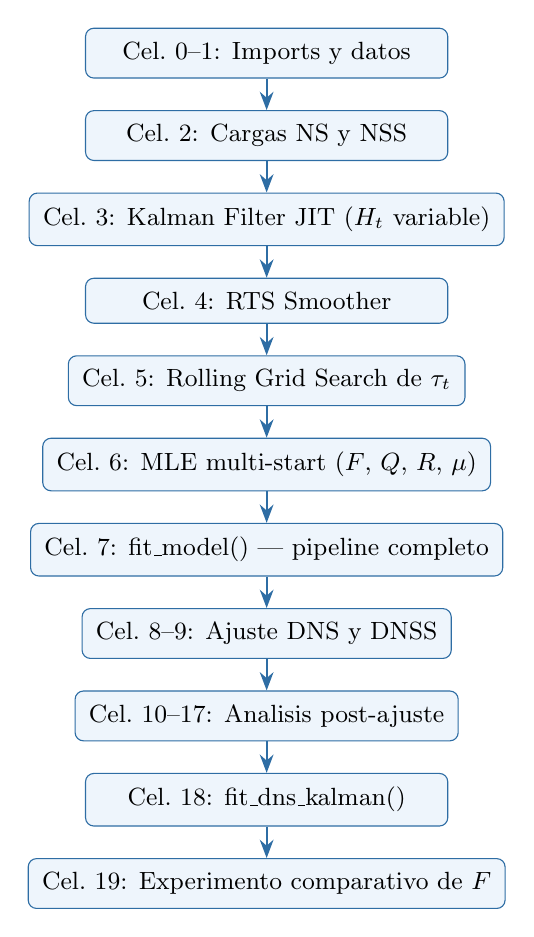
\begin{tikzpicture}[
  node distance=0.4cm and 1.4cm,
  box/.style={
    rectangle, rounded corners=3pt,
    draw=azulmedio, fill=azulmuyclaro,
    font=\small, inner sep=5pt,
    minimum width=4.6cm, minimum height=0.55cm
  },
  arr/.style={-Stealth, azulmedio, line width=0.8pt}
]
  \node[box] (c0) {Cel.\ 0--1: Imports y datos};
  \node[box, below=of c0] (c1) {Cel.\ 2: Cargas NS y NSS};
  \node[box, below=of c1] (c2) {Cel.\ 3: Kalman Filter JIT ($H_t$ variable)};
  \node[box, below=of c2] (c3) {Cel.\ 4: RTS Smoother};
  \node[box, below=of c3] (c4) {Cel.\ 5: Rolling Grid Search de $\tau_t$};
  \node[box, below=of c4] (c5) {Cel.\ 6: MLE multi-start ($F$, $Q$, $R$, $\mu$)};
  \node[box, below=of c5] (c6) {Cel.\ 7: fit\_model() — pipeline completo};
  \node[box, below=of c6] (c7) {Cel.\ 8--9: Ajuste DNS y DNSS};
  \node[box, below=of c7] (c8) {Cel.\ 10--17: Analisis post-ajuste};
  \node[box, below=of c8] (c9) {Cel.\ 18: fit\_dns\_kalman()};
  \node[box, below=of c9] (c10){Cel.\ 19: Experimento comparativo de $F$};
  \foreach \a/\b in {c0/c1,c1/c2,c2/c3,c3/c4,c4/c5,c5/c6,
                     c6/c7,c7/c8,c8/c9,c9/c10}
    \draw[arr] (\a)--(\b);
\end{tikzpicture}
\end{center}

% ═════════════════════════════════════════════════════════════
\section{Modelo espacio-estado}
\label{sec:modelo}
% ═════════════════════════════════════════════════════════════

\subsection{Formulacion general}

\begin{teoremabox}{Modelo espacio-estado DNS/DNSS con $H_t$ variable}
\textbf{Ecuacion de observacion:}
\begin{equation}
  \by_t = \bH(\tau_t)\,\bbet_t + \beps_t, \qquad
  \beps_t \sim \N(\bzero,\,\bR),
  \qquad t = 1,\ldots,T
  \label{eq:obs}
\end{equation}

\textbf{Ecuacion de transicion:}
\begin{equation}
  \bbet_t = \bmu + \bF(\bbet_{t-1} - \bmu) + \bm{\eta}_t, \qquad
  \bm{\eta}_t \sim \N(\bzero,\,\bQ)
  \label{eq:trans}
\end{equation}

donde $\by_t \in \mathbb{R}^N$ son rendimientos en $N$ plazos,
$\bbet_t \in \mathbb{R}^k$ son factores latentes ($k=3$ DNS, $k=4$ DNSS),
$\bH_t = \bH(\tau_t) \in \mathbb{R}^{N \times k}$ son cargas
\textbf{variables en el tiempo} (la clave del metodo),
$\bmu \in \mathbb{R}^k$ es la media de largo plazo de los factores,
$\bF \in \mathbb{R}^{k \times k}$ la matriz de transicion,
$\bR = \diag(r_1,\ldots,r_N)$ y $\bQ = \diag(q_1,\ldots,q_k)$ matrices diagonales.
\end{teoremabox}

\begin{notabox}[Innovacion central: $H_t$ variable]
A diferencia del Filtro de Kalman estandar donde $\bH$ es constante,
aqui $\bH_t = \bH(\tau_t)$ cambia en cada periodo porque $\tau_t$ fue
seleccionado por Grid Search en ese periodo. Esto requiere que el KF reciba
un array $(T \times N \times k)$ en lugar de una matriz fija $(N \times k)$.
El algoritmo sigue siendo lineal y gaussiano en cada $t$ dado $\tau_t$,
por lo que las ecuaciones del KF son exactas.
\end{notabox}

\subsection{Cargas Nelson-Siegel (DNS, $k=3$)}

La funcion de carga de NS mapea cada plazo $m_n$ a tres pesos:
\begin{equation}
  \bH_n(\tau_1) = \left[
    1,\quad
    \frac{1-e^{-m_n/\tau_1}}{m_n/\tau_1},\quad
    \frac{1-e^{-m_n/\tau_1}}{m_n/\tau_1} - e^{-m_n/\tau_1}
  \right]
  \label{eq:ns}
\end{equation}

\begin{itemize}[leftmargin=1.5em, itemsep=2pt]
  \item $\beta_{0,t}$: \textbf{nivel} --- carga constante $=1$;
        determina la tasa de largo plazo $\lim_{m\to\infty}y_t(m)=\beta_{0,t}$.
  \item $\beta_{1,t}$: \textbf{pendiente} --- carga decreciente de 1 a 0;
        captura el spread largo-corto $y_t(\infty) - y_t(0^+) = \beta_{0,t} - (\beta_{0,t}+\beta_{1,t})$.
  \item $\beta_{2,t}$: \textbf{curvatura} --- carga en forma de campana con
        maximo en $m^* \approx 1.793\,\tau_1$.
\end{itemize}

\subsection{Cargas Nelson-Siegel-Svensson (DNSS, $k=4$)}

Svensson (1994) extiende NS con un cuarto factor de curvatura independiente:
\begin{equation}
  \bH_n(\tau_1,\tau_2) = \left[
    \bH_n(\tau_1),\quad
    \frac{1-e^{-m_n/\tau_2}}{m_n/\tau_2} - e^{-m_n/\tau_2}
  \right]
  \label{eq:nss}
\end{equation}

$\beta_{3,t}$ es una segunda curvatura con hump en $m^{**} \approx 1.793\,\tau_2$.
Esto permite capturar formas de curva con dos jorobas o primas de plazo
en el tramo largo que NS no puede representar.

\textbf{Restriccion de separacion:} se impone $|\tau_1 - \tau_2| \geq 0.15$
para evitar colinealidad en las columnas de $\bH$ que causaria mal
condicionamiento en el OLS del Grid Search.

\subsection{Interpretacion de $\tau$ y el hump}

El parametro $\tau$ controla donde se ubica el maximo de la carga de curvatura:
\begin{equation}
  m^*(\tau) \approx 1.793\,\tau \quad \text{anos}
  \label{eq:hump}
\end{equation}

Para curvas de Tesoros de EEUU, el hump tipicamente se ubica entre 2 y 5 anos
($\tau_1 \approx 1.1$--$2.8$). Para TES Colombia el rango es similar aunque
puede variar con los ciclos de politica monetaria del Banco de la Republica.
El Grid Search re-estima $\tau_t$ en cada periodo para seguir estos cambios.

\subsection{Estructura de la matriz $\bF$}

\begin{table}[H]
\centering
\caption{Estructuras disponibles para la matriz de transicion $\bF$}
\label{tab:F}
\small
\begin{tabular}{L{2.2cm} C{1.8cm} L{5.5cm} L{3.5cm}}
\toprule
\textbf{F\_type}
  & \textbf{Parametros}
  & \textbf{Interpretacion economica}
  & \textbf{Referencia} \\
\midrule
\texttt{'diagonal'}
  & $k$
  & Cada factor sigue un AR(1) independiente. Ortogonalidad de los shocks.
  & Caldeira et al.\ (2010) P7, Cakmaklı (2013) \\
\addlinespace
\texttt{'triangular'}
  & $k(k+1)/2$
  & Nivel influye en pendiente y curvatura (jerarquia causal). Off-diagonals libres en el triangulo inferior.
  & Extension propia \\
\addlinespace
\texttt{'completa'}
  & $k^2$
  & VAR(1) irrestricto. Maxima flexibilidad. Requiere verificar estabilidad ($|\lambda_i| < 1$).
  & VAR(1) general \\
\bottomrule
\end{tabular}
\end{table}

\begin{tipbox}[Eleccion de F\_type]
La literatura empirica (Caldeira et al.\ 2010, Cakmaklı 2013) reporta
diferencias de RMSE $< 0.4\,\text{pb}$ entre la especificacion diagonal (P7)
y el VAR completo (P6). La diagonal es preferible por parsimonia y menor
riesgo de sobreajuste, especialmente en muestras de tamano moderado.
Para TES Colombia con $T \approx 150$--$300$ observaciones mensuales,
se recomienda empezar con \texttt{'diagonal'}.
\end{tipbox}

% ═════════════════════════════════════════════════════════════
\section{Rolling Grid Search de $\tau_t$}
\label{sec:gridsearch}
% ═════════════════════════════════════════════════════════════

\subsection{Fundamento: por que re-estimar $\tau$ en el tiempo}

El enfoque de Diebold \& Li (2006) fija $\tau$ en un valor unico
(tipicamente $\tau = 1.5$ anos) para toda la muestra.
Esto es incorrecto cuando la forma de la curva cambia sistematicamente,
como ocurre en periodos de cambio de regimen monetario.

El Grid Search por ventana estima, para cada periodo $t$:
\begin{equation}
  \hat{\tau}_t = \arg\min_{\tau \in \mathcal{G}}\;
    \text{SSE}(\tau;\, \mathcal{W}_t)
  \label{eq:gridsearch}
\end{equation}

donde $\mathcal{G}$ es la cuadricula de candidatos y
$\mathcal{W}_t$ es la ventana de observaciones usada para evaluar el ajuste.

\subsection{Reformulacion via Residual Maker}

El SSE de minimos cuadrados de NS en la ventana $\mathcal{W}_t$ puede
reescribirse de forma que se \emph{desacopla} el calculo entre $\tau$
(dependiente del candidato) y los datos (dependientes del periodo):

\begin{teoremabox}{Reformulacion del SSE con Residual Maker}
Para un candidato $\tau$ fijo, el SSE de OLS sobre la ventana $\mathcal{W}_t$ es:
\begin{equation}
  \text{SSE}(\tau,\, t) = \tr\!\left(M_\tau\,\Sigma_t\right)
  \label{eq:sse_trace}
\end{equation}
donde:
\begin{align}
  M_\tau &= \bI - \bH(\tau)\!\left[\bH(\tau)^\top\bH(\tau)\right]^{-1}\!\bH(\tau)^\top
  \quad \text{(residual maker, $(N \times N)$)}
  \label{eq:resmaker} \\
  \Sigma_t &= \sum_{s \in \mathcal{W}_t} \by_s\,\by_s^\top
  \quad \text{(matriz acumulada de productos cruzados, $(N \times N)$)}
  \label{eq:sigma_t}
\end{align}
\end{teoremabox}

$M_\tau$ es el proyector ortogonal al espacio columna de $\bH(\tau)$.
Es simetrico ($M_\tau = M_\tau^\top$) e idempotente ($M_\tau^2 = M_\tau$).

\textbf{Eficiencia computacional:}
\begin{itemize}[leftmargin=1.5em, itemsep=2pt]
  \item $M_\tau$ se precalcula \textbf{una sola vez} por candidato $\tau \in \mathcal{G}$,
        antes del bucle temporal.
  \item $\Sigma_t$ se actualiza incrementalmente mediante
        \textbf{sumas de prefijo acumuladas}: $\Sigma_t = \Sigma_{t-1} + \by_t\,\by_t^\top$
        (ventana expandiente) o $\Sigma_t = \Sigma_{t-1} + \by_t\by_t^\top - \by_{t-W}\by_{t-W}^\top$
        (ventana rodante de tamano $W$).
  \item La evaluacion del SSE por candidato en cada periodo es simplemente
        $\tr(M_\tau\,\Sigma_t)$, implementada con \texttt{einsum} en NumPy:
\end{itemize}

\begin{codigocaja}{Celda 5 --- vectorizacion con einsum}
# M_arr : (G, N, N)  residual makers precomputados
# Sigma : (N, N)     matriz de productos cruzados de la ventana actual

# Evalua SSE para todos los candidatos simultaneamente:
sse_vec = np.einsum('gij,ji->g', M_arr, Sigma)  # (G,) en O(G*N^2)
best_g  = np.argmin(sse_vec)
tau1_t  = tau1_grid[best_g]
\end{codigocaja}

\textbf{Complejidad computacional:}
La formulacion con residual maker reduce la complejidad de
$O(|\mathcal{G}| \cdot T \cdot (Nk^2 + N^2k))$ (OLS en cada $t$) a
$O(|\mathcal{G}| \cdot N^2)$ de precalculo +
$O(|\mathcal{G}| \cdot T \cdot N^2)$ de evaluacion,
con la actualización de $\Sigma_t$ en $O(N^2)$ por periodo.

\subsection{Ventana rodante vs expandiente}

La ventana $\mathcal{W}_t$ determina que datos se usan para elegir $\tau_t$:

\begin{table}[H]
\centering
\caption{Tipos de ventana para el Grid Search}
\label{tab:ventana}
\small
\begin{tabular}{L{2.5cm} L{4.5cm} L{4cm} L{3cm}}
\toprule
\textbf{window\_size}
  & \textbf{Datos usados}
  & \textbf{Ventajas}
  & \textbf{Limitaciones} \\
\midrule
\texttt{None}
  & $[1, t]$ --- toda la historia
  & Causalmente correcta; $\tau_t$ estable; optima para pronostico
  & Poca reactividad a cambios recientes \\
\addlinespace
$W$ entero
  & $[t-W+1, t]$ --- ultimas $W$ obs
  & Reactiva a cambios de regimen; captura estructuras locales
  & Mayor varianza de $\tau_t$; sensible a outliers \\
\bottomrule
\end{tabular}
\end{table}

\textbf{Recomendacion practica:}
Para datos semanales de TES Colombia, usar $W \approx 52$ (un ano)
como punto de partida. Para datos mensuales, $W \approx 36$--$60$.
Explorar la sensibilidad a $W$ mediante el perfil SSE
(disponible en \texttt{plot\_perfil\_sse\_tau()}).

\subsection{Grid Search 2D para DNSS}

Para DNSS, la cuadricula es bidimensional $\mathcal{G}_1 \times \mathcal{G}_2$
y la reformulacion del SSE requiere el residual maker conjunto:

\begin{equation}
  M_{\tau_1,\tau_2} = \bI - \bH(\tau_1,\tau_2)
    \left[\bH(\tau_1,\tau_2)^\top\bH(\tau_1,\tau_2)\right]^{-1}
    \bH(\tau_1,\tau_2)^\top
  \label{eq:resmaker2d}
\end{equation}

El array de residual makers tiene dimension $(G_1 \times G_2 \times N \times N)$
y la evaluacion vectorizada usa:

\begin{codigocaja}{Celda 5 --- Grid Search 2D para DNSS}
# M_arr : (G1, G2, N, N) residual makers precomputados
# Sigma : (N, N)

sse_grid = np.einsum('ghjk,kj->gh', M_arr, Sigma)  # (G1, G2)
sse_grid[~valid] = np.inf   # marcar combinaciones invalidas
flat_best = np.argmin(sse_grid.ravel())
bi, bj    = np.unravel_index(flat_best, (G1, G2))
tau1_t, tau2_t = tau1_grid[bi], tau2_grid[bj]
\end{codigocaja}

\begin{atencionbox}[OLS SSE $\neq$ log-verosimilitud marginal]
El Grid Search minimiza el SSE de OLS en dos etapas (Diebold-Li two-step),
que puede seleccionar un $\tau$ distinto al optimo de la
log-verosimilitud marginal del Filtro de Kalman.
La diferencia puede ser de miles de puntos de log-lik.
Sin embargo, el Grid Search es causalmente correcto y computacionalmente
eficiente, lo que lo hace adecuado para el proposito de inicializar $H_t$.
Los parametros del proceso de estado $(F, Q, R, \mu)$ se estiman
correctamente por MLE en el paso siguiente.
\end{atencionbox}

% ═════════════════════════════════════════════════════════════
\section{Filtro de Kalman con $H_t$ variable}
\label{sec:kf}
% ═════════════════════════════════════════════════════════════

\subsection{Algoritmo completo}

\begin{algoritmo}[Kalman Filter con cargas variables --- \texttt{\_kf\_core()}]
\label{alg:kf}
Dado $\bm{\theta} = (\bmu, \bF, \bQ, \bR)$ y $\{H_t\}_{t=1}^T$,
computar estados filtrados y log-verosimilitud.

\textbf{Inicializacion:} $\hat{\bbet}_{0|0} = \bmu$,
$\bP_{0|0}$ estacionaria (ecuacion de Lyapunov).

Para $t = 1, \ldots, T$:

\textbf{Prediccion:}
\begin{align}
  \hat{\bbet}_{t|t-1} &= \bmu + \bF\!\left(\hat{\bbet}_{t-1|t-1} - \bmu\right)
  \label{eq:pred_state} \\
  \bP_{t|t-1} &= \bF\,\bP_{t-1|t-1}\,\bF^\top + \bQ
  \label{eq:pred_cov}
\end{align}

\textbf{Innovacion y varianza de innovacion:}
\begin{align}
  \bv_t &= \by_t - \bH_t\,\hat{\bbet}_{t|t-1}
  \label{eq:innov} \\
  \bS_t &= \bH_t\,\bP_{t|t-1}\,\bH_t^\top + \bR
  \label{eq:innov_cov}
\end{align}

\textbf{Contribucion a la log-verosimilitud} (via descomposicion de Cholesky):
\begin{equation}
  \ell_t = -\frac{N}{2}\log(2\pi)
           - \frac{1}{2}\!\underbrace{\sum_{n=1}^N 2\log L_{t,nn}}_{\log|\bS_t|}
           - \frac{1}{2}\underbrace{\|\bL_t^{-1}\bv_t\|^2}_{\bv_t^\top \bS_t^{-1}\bv_t}
  \label{eq:loglik_t}
\end{equation}
donde $\bL_t$ es la factorizacion de Cholesky: $\bS_t = \bL_t\bL_t^\top$.

\textbf{Actualizacion} (forma Joseph):
\begin{align}
  \bK_t &= \bP_{t|t-1}\,\bH_t^\top\,\bS_t^{-1}
  \label{eq:gain} \\
  \hat{\bbet}_{t|t} &= \hat{\bbet}_{t|t-1} + \bK_t\,\bv_t
  \label{eq:update_state} \\
  \bP_{t|t} &= (\bI - \bK_t\bH_t)\,\bP_{t|t-1}\,(\bI - \bK_t\bH_t)^\top
               + \bK_t\bR\bK_t^\top
  \label{eq:joseph}
\end{align}

Log-verosimilitud total: $\log\mathcal{L} = \sum_{t=1}^T \ell_t$.
\end{algoritmo}

\subsection{Por que la forma Joseph (ecuacion~\ref{eq:joseph})}

La forma estandar de actualizacion de covarianza es $(I-KH)P$, que equivale
a la forma Joseph pero con menos operaciones. Sin embargo, la forma estandar
pierde la simetria numerica de $P_{t|t}$ cuando la ganancia $K_t$ es grande
(filtro muy activo). La forma Joseph garantiza que:
\begin{equation}
  \bP_{t|t} = \bP_{t|t}^\top \quad \text{y} \quad
  \bP_{t|t} \succ \bzero
  \quad \text{en todo } t
  \label{eq:joseph_property}
\end{equation}

Esto es esencial en series largas (TES Colombia con $T > 500$ observaciones
diarias) donde los errores de redondeo de la forma estandar pueden
acumularse y hacer $P_{t|t}$ indefinida.

\subsection{Cholesky para log-det y cuadratica}

El calculo del log-determinante y la forma cuadratica
$\bv_t^\top \bS_t^{-1}\bv_t$ nunca forma $\bS_t^{-1}$ explicitamente.
En cambio, se resuelve mediante la factorizacion de Cholesky:
\begin{align}
  \bS_t &= \bL_t\bL_t^\top \quad \Rightarrow \quad
  \log|\bS_t| = 2\sum_{n=1}^N \log(L_{t,nn})
  \label{eq:chol_det} \\
  \bz_t &= \bL_t^{-1}\bv_t \quad \Rightarrow \quad
  \bv_t^\top\bS_t^{-1}\bv_t = \|\bz_t\|^2
  \label{eq:chol_quad}
\end{align}

Esto es numericamente estable incluso cuando $\bS_t$ esta mal condicionada.
La ganancia de Kalman se calcula analogamente: $\bK_t = \bS_t^{-1}(\bH_t\bP_{t|t-1})^\top$
mediante dos triangular solves.

\subsection{Inicializacion estacionaria}

La covarianza inicial $\bP_{0|0}$ se obtiene como la solucion de la
ecuacion de Lyapunov discreta $\bP = \bF\bP\bF^\top + \bQ$:
\begin{equation}
  P_{0,ii} = \frac{q_i}{1 - f_i^2}, \qquad
  P_{0,ij} = 0 \quad (i \neq j)
  \quad \text{para } \bF \text{ diagonal}
  \label{eq:p0}
\end{equation}

Para $\bF$ triangular o completa se usa \texttt{scipy.linalg.solve\_discrete\_lyapunov()}.

\subsection{Implementacion con Numba JIT}

La funcion \texttt{\_kf\_core()} esta compilada con Numba JIT para maxima velocidad.
Acepta el array $(T \times N \times k)$ de cargas variables:

\begin{codigocaja}{Celda 3 --- firma de \_kf\_core() y wrapper}
# Firma del KF compilado (Numba JIT cuando esta disponible):
def _kf_core(yields,   # (T, N) rendimientos observados
             H_arr,    # (T, N, k) cargas variables en t
             F,        # (k, k) transicion
             Q,        # (k, k) cov. innovaciones de estado
             R_diag,   # (N,)   varianzas de medicion
             mu,       # (k,)   media de largo plazo
             beta0,    # (k,)   estado inicial
             P0):      # (k, k) covarianza inicial
    # Retorna:
    # beta_pred : (T, k)    beta_{t|t-1}
    # beta_filt : (T, k)    beta_{t|t}
    # P_pred    : (T, k, k) P_{t|t-1}
    # P_filt    : (T, k, k) P_{t|t}
    # innov     : (T, N)    innovaciones v_t
    # loglik    : float     log-verosimilitud total
    ...
\end{codigocaja}

% ═════════════════════════════════════════════════════════════
\section{Suavizador RTS (Rauch-Tung-Striebel)}
\label{sec:rts}
% ═════════════════════════════════════════════════════════════

\subsection{Que aporta el suavizador}

El Filtro de Kalman produce estados \textbf{filtrados}
$\hat{\bbet}_{t|t} = \E{\bbet_t \mid \bY_{1:t}}$:
la mejor estimacion de $\bbet_t$ dado lo que se observa hasta $t$.
Son causalmente correctos pero tienen mayor varianza porque no usan
informacion futura.

El Suavizador RTS produce estados \textbf{suavizados}
$\hat{\bbet}_{t|T} = \E{\bbet_t \mid \bY_{1:T}}$:
la mejor estimacion usando \emph{toda} la muestra.
Son preferibles para analisis historico y diagnostico in-sample.

\subsection{Algoritmo backward}

\begin{algoritmo}[RTS Smoother --- \texttt{rts\_smoother()}]
\label{alg:rts}
Usando los resultados del KF forward:

\textbf{Inicializacion:}
$\hat{\bbet}_{T|T}$, $\bP_{T|T}$ (del filtro).

Para $t = T-1, T-2, \ldots, 1$:
\begin{align}
  \bG_t &= \bP_{t|t}\,\bF^\top\,\bP_{t+1|t}^{-1}
  \quad \text{(ganancia suavizadora)}
  \label{eq:smooth_gain} \\
  \hat{\bbet}_{t|T} &= \hat{\bbet}_{t|t}
    + \bG_t\!\left(\hat{\bbet}_{t+1|T} - \hat{\bbet}_{t+1|t}\right)
  \label{eq:smooth_state} \\
  \bP_{t|T} &= \bP_{t|t}
    + \bG_t\!\left(\bP_{t+1|T} - \bP_{t+1|t}\right)\bG_t^\top
  \label{eq:smooth_cov}
\end{align}
\end{algoritmo}

\begin{notabox}[El RTS es independiente de $H_t$]
El suavizador RTS opera en el espacio de \emph{estados} $\bbet_t$,
no en el espacio de observaciones. Por lo tanto, sus ecuaciones
(~\ref{eq:smooth_gain}--\ref{eq:smooth_cov}) solo dependen de $\bF$ y $\bQ$,
y son validas aunque las cargas $H_t$ varien en el tiempo.
Esto es una propiedad elegante del modelo espacio-estado lineal gaussiano.
\end{notabox}

La ganancia suavizadora $\bG_t = \bP_{t|t}\,\bF^\top\,\bP_{t+1|t}^{-1}$
puede interpretarse como cuanta informacion futura (la diferencia
$\hat{\bbet}_{t+1|T} - \hat{\bbet}_{t+1|t}$) se propaga hacia atras al
revisar la estimacion de $\bbet_t$. Un $\bG_t$ grande indica que el estado
pasado debe revisarse significativamente dados los datos futuros.

% ═════════════════════════════════════════════════════════════
\section{Estimacion MLE multi-start}
\label{sec:mle}
% ═════════════════════════════════════════════════════════════

\subsection{Problema de optimizacion}

Dados $\{H_t\}_{t=1}^T$ del Grid Search, los parametros del proceso de estado
$\bm{\theta} = (\bmu, \bF, \bQ, \bR)$ se estiman maximizando la
log-verosimilitud del Filtro de Kalman:
\begin{equation}
  \hat{\bm{\theta}} =
  \arg\max_{\bm{\theta}}\; \log\mathcal{L}(\bm{\theta} \mid \bY,\, \{H_t\})
  = \arg\max_{\bm{\theta}}\; \sum_{t=1}^T \ell_t(\bm{\theta})
  \label{eq:mle}
\end{equation}

El problema es no convexo: la superficie de log-verosimilitud puede tener
multiples optimos locales, especialmente cuando $F$ es triangular o completa.
La solucion es el \textbf{multi-start}: ejecutar L-BFGS-B desde $n_\text{starts}$
puntos aleatorios y retener el mejor.

\subsection{Parametrizacion sin restricciones}

Para garantizar que las restricciones de positividad y estabilidad siempre
se cumplan durante la optimizacion, los parametros se transforman antes
de pasarlos al optimizador:

\begin{table}[H]
\centering
\caption{Reparametrizacion para la optimizacion sin restricciones}
\label{tab:reparam}
\small
\begin{tabular}{L{2.8cm} L{3cm} L{3.5cm} L{4cm}}
\toprule
\textbf{Parametro}
  & \textbf{Restriccion}
  & \textbf{Transformacion}
  & \textbf{Inversa} \\
\midrule
$f_{ii}$ (diagonal $F$)
  & $|f_{ii}| < 0.995$
  & $x_i = \text{arctanh}(f_{ii}/0.995)$
  & $f_{ii} = 0.995\tanh(x_i)$ \\
\addlinespace
$f_{ij}$ ($i > j$, triangular)
  & libre
  & $x_{ij} = f_{ij}$
  & $f_{ij} = x_{ij}$ \\
\addlinespace
$q_i$ (diagonal $Q$)
  & $q_i > 0$
  & $x_i = \log(q_i)$
  & $q_i = e^{x_i}$ \\
\addlinespace
$r_n$ (diagonal $R$)
  & $r_n > 0$
  & $x_n = \log(r_n)$
  & $r_n = e^{x_n}$ \\
\addlinespace
$\mu_i$
  & libre
  & $x_i = \mu_i$
  & $\mu_i = x_i$ \\
\bottomrule
\end{tabular}
\end{table}

El limite $|f_{ii}| < 0.995$ (no exactamente 1) garantiza que los
eigenvalores de $\bF$ esten dentro del circulo unitario, asegurando
estacionariedad del proceso de estado. Usar $\tanh$ en lugar de $\text{clip}$
produce gradientes continuos que el optimizador puede usar.

\subsection{Numero de parametros por configuracion}

\begin{table}[H]
\centering
\caption{Parametros libres en la MLE segun model y F\_type}
\label{tab:nparams}
\small
\begin{tabular}{cccccc}
\toprule
\textbf{model} & $k$ & \textbf{F\_type} & \textbf{Params en $F$}
  & \textbf{Params $\mu,Q,R$} & \textbf{Total} \\
\midrule
DNS  & 3 & diagonal   & 3            & $3+3+N$ & $9+N$ \\
DNS  & 3 & triangular & 6            & $3+3+N$ & $12+N$ \\
DNS  & 3 & completa   & 9            & $3+3+N$ & $15+N$ \\
DNSS & 4 & diagonal   & 4            & $4+4+N$ & $12+N$ \\
DNSS & 4 & triangular & 10           & $4+4+N$ & $18+N$ \\
DNSS & 4 & completa   & 16           & $4+4+N$ & $24+N$ \\
\bottomrule
\end{tabular}
\end{table}

\textbf{Criterios de informacion} usados para comparar modelos:
\begin{align}
  \text{AIC} &= -2\log\mathcal{L} + 2p
  \label{eq:aic} \\
  \text{BIC} &= -2\log\mathcal{L} + p\log T
  \label{eq:bic}
\end{align}
donde $p$ es el numero de parametros libres.

\subsection{Extensiones para plazos largos}

\subsubsection{Opcion A --- $R$ estructurada por grupos}

Reduce $N$ varianzas a 3 parametros (corto/medio/largo):
\begin{equation}
  r_n = r_{g(n)}, \qquad
  g(n) = \begin{cases}
    \text{corto} & m_n \leq \text{th}_1 \\
    \text{medio} & \text{th}_1 < m_n \leq \text{th}_2 \\
    \text{largo} & m_n > \text{th}_2
  \end{cases}
  \label{eq:r_grupos}
\end{equation}

En el MLE se optimizan solo 3 parametros de $R$ en lugar de $N$,
reduciendo el riesgo de sobreajuste y reflejando la estructura economica
del mercado (los spreads de liquidez varian por tramo).

\subsubsection{Opcion C --- Pesos en la log-verosimilitud}

Escala inversamente las varianzas de medicion antes del KF:
$r_n^\text{eff} = r_n / w_n$. Un peso $w_n > 1$ hace que el filtro
confie mas en el plazo $n$, lo que fuerza al MLE a ajustarlo mejor:
\begin{equation}
  \log\mathcal{L}^{(w)} =
  \sum_{t=1}^T \sum_{n=1}^N
  -\frac{1}{2}\!\left[\log(2\pi r_n / w_n) + \frac{v_{t,n}^2}{r_n/w_n}\right]
  \label{eq:loglik_weighted}
\end{equation}

Esta es una cuasi-maxima verosimilitud ponderada: el investigador asigna
mayor importancia a ajustar bien ciertos plazos.

% ═════════════════════════════════════════════════════════════
\section{Analisis post-ajuste}
\label{sec:postfit}
% ═════════════════════════════════════════════════════════════

El notebook genera automaticamente seis bloques de diagnostico,
todos accesibles tambien de forma individual.

\subsection{Factores latentes --- \texttt{plot\_factores()}}

Grafica los estados \textbf{filtrados} $\hat{\bbet}_{t|t}$ y
\textbf{suavizados} $\hat{\bbet}_{t|T}$ para cada factor con
bandas de confianza al 95\% basadas en la diagonal de $\bP_{t|T}$:
\begin{equation}
  \hat{\bbet}_{i,t|T} \pm 1.96\,\sqrt{P_{t|T,ii}}
  \label{eq:ic_factors}
\end{equation}

El diferencial entre filtrado y suavizado es diagnosticamente util:
una diferencia grande indica que el modelo revisa sustancialmente
su estimacion del estado pasado al recibir datos futuros, lo que
puede senalar mal especificacion en la dinamica de transicion.

Se reportan ademas:
\begin{itemize}[leftmargin=1.5em, itemsep=2pt]
  \item Estadisticos descriptivos: media, std, percentiles.
  \item Autocorrelaciones a lag 1 y lag 5 como medida de persistencia.
\end{itemize}

\subsection{Evolucion de $\tau_t$ --- \texttt{plot\_tau\_evolution()}}

Muestra la serie temporal de $\tau_t$ con la ubicacion del hump
$m^*_t = 1.793\,\tau_t$ en el eje secundario.
Incluye banda de percentiles P10--P90 y distribucion marginal con KDE.

Una alta variabilidad en $\tau_t$ indica que la forma de la curva
cambia significativamente en el tiempo. Para TES Colombia esto es
esperado dado los distintos regimenes monetarios del Banco de la Republica.

\subsection{Curva ajustada --- \texttt{plot\_curvas\_ajustadas()}}

Superpone la curva observada (puntos) con la curva ajustada (linea continua)
en $n$ fechas seleccionadas uniformemente. La curva ajustada se evalua
en una malla fina de 200 puntos usando el estado suavizado:
$\hat{y}_t(m) = \bH(m;\, \tau_t)^\top \hat{\bbet}_{t|T}$.

\subsection{Residuos de medicion --- \texttt{analisis\_residuos()}}

Cuatro niveles de diagnostico:

\begin{enumerate}[leftmargin=1.5em]
  \item \textbf{RMSE y MAE por plazo}: identifica donde falla el modelo.
        Tipicamente los plazos cortos (poca liquidez) y largos (prima de plazo)
        tienen mayor error que los intermedios.
  \item \textbf{Sesgo medio por plazo}: sesgo positivo = subestimacion sistematica.
        Un sesgo grande en el plazo largo indica que la estructura factorial
        no captura la prima de plazo.
  \item \textbf{Correlacion cruzada de residuos}: si los residuos de distintos
        plazos estan correlacionados, el modelo omite un factor comun.
        Alta correlacion entre residuos 20Y y 30Y es tipica cuando hay una
        prima de plazo no modelada.
  \item \textbf{Tests estadisticos}: Jarque-Bera (normalidad) y Ljung-Box lag 10
        (autocorrelacion serial) por plazo. LB $p < 0.05$ indica patrones
        seriales residuales que sugieren mal especificacion.
\end{enumerate}

\subsection{Diagnosticos del filtro --- \texttt{diagnosticos\_filtro()}}

\begin{teoremabox}{Condicion de especificacion correcta del KF}
Un Filtro de Kalman correctamente especificado produce innovaciones
\textbf{blancas} y \textbf{normalizadas}:
\begin{equation}
  \tilde{v}_{t,n} = \frac{v_{t,n}}{\hat{\sigma}_n} \sim \N(0,1) \quad \text{i.i.d.}
  \label{eq:white_innov}
\end{equation}
Si hay autocorrelacion en las innovaciones, el modelo esta mal especificado
(por ejemplo, la dinamica de transicion o las cargas son insuficientemente flexibles).
\end{teoremabox}

Se reportan:
\begin{itemize}[leftmargin=1.5em, itemsep=2pt]
  \item Series temporales de $\tilde{v}_{t,n}$ con marcado de outliers
        ($|\tilde{v}| > 2.58\,\sigma$).
  \item Histograma con curva $\N(0,1)$ teorica.
  \item Log-verosimilitud acumulada: una ruptura en su pendiente puede
        indicar un cambio de regimen.
  \item Test de Ljung-Box lag 10 sobre las innovaciones normalizadas.
\end{itemize}

\subsection{Parametros MLE --- \texttt{resumen\_parametros()}}

\begin{itemize}[leftmargin=1.5em, itemsep=2pt]
  \item $\bmu$: media de largo plazo de los factores. Bajo especificacion
        correcta, $\bbet_t$ revierte a $\bmu$ en el largo plazo.
  \item $\bF$: heatmap con eigenvalores graficados en el circulo unitario.
        Un eigenvalor fuera del circulo indica inestabilidad.
  \item \textbf{Semividas implicitas}: $h_i = -\log(2)/\log(|f_{ii}|)$ periodos.
        Indica cuanto tarda cada factor en reducir su desviacion respecto a $\mu_i$
        a la mitad.
  \item $\sigma_{\eta,i} = \sqrt{q_i}$ y $\sigma_{\varepsilon,n} = \sqrt{r_n}$
        en puntos basicos.
\end{itemize}

\subsection{Perfil SSE de $\tau$ --- \texttt{plot\_perfil\_sse\_tau()}}

Heatmap del perfil SSE normalizado en el tiempo para DNS:
los candidatos $\tau \in \mathcal{G}$ en el eje vertical,
el tiempo en el eje horizontal, y la intensidad representa el SSE
(amarillo = bajo SSE = candidato preferido).
Superpone la trayectoria $\hat{\tau}_t$ seleccionada en cada periodo.
Diagnostica la robustez de la seleccion de $\tau$: un perfil SSE
muy plano indica que muchos valores de $\tau$ tienen ajuste similar,
lo que sugiere poca identificacion de la curvatura en ese periodo.

% ═════════════════════════════════════════════════════════════
\section{Documentacion de funciones}
\label{sec:funciones}
% ═════════════════════════════════════════════════════════════

\subsection{Cargas}

\begin{codigocaja}{Celda 2 --- ns\_loadings(), nss\_loadings(), get\_H()}
def ns_loadings(maturities, tau1):
    '''Cargas Nelson-Siegel. Shape (N, 3). [nivel, pendiente, curvatura].'''
    m  = np.asarray(maturities, dtype=float)
    mt = m / tau1; e = np.exp(-mt); c = (1.0 - e) / mt
    return np.column_stack([np.ones_like(m), c, c - e])

def nss_loadings(maturities, tau1, tau2):
    '''Cargas Nelson-Siegel-Svensson. Shape (N, 4).
    Requiere |tau1 - tau2| >= 0.15 para evitar colinealidad.'''
    ...

def get_H(maturities, tau1, tau2, model):
    '''Wrapper: model="DNS" -> ns_loadings | "DNSS" -> nss_loadings.'''
    ...
\end{codigocaja}

\subsection{Grid Search}

\begin{codigocaja}{Celda 5 --- Grid Search de tau\_t}
# Residual maker (precomputado una vez por candidato):
M = _residual_maker(H)              # M = I - H(H'H)^{-1}H', shape (N, N)

# Sumas acumuladas de y_s y_s' (precomputadas una vez):
YYt_cum = _build_YYt_cumsum(yields) # shape (T+1, N, N)

# DNS: Grid Search 1D
tau1_t, sse_t, sse_grid = rolling_tau_dns(
    yields, maturities,
    tau1_grid   = np.linspace(0.5, 5.0, 35),
    window_size = 52)              # None -> ventana expandiente

# DNSS: Grid Search 2D
tau1_t, tau2_t, sse_t = rolling_tau_dnss(
    yields, maturities,
    tau1_grid   = np.linspace(0.5, 5.0, 22),
    tau2_grid   = np.linspace(0.15, 3.0, 18),
    window_size = 52,
    sep_min     = 0.15)            # separacion minima |tau1 - tau2|

# Construir array de cargas (T, N, k) a partir de tau_t:
H_arr = build_H_array(maturities, tau1_t, tau2_t, model='DNSS')
\end{codigocaja}

\subsection{Kalman Filter y RTS}

\begin{codigocaja}{Celdas 3-4 --- KF y RTS}
# Kalman Filter con H_t variable:
beta_pred, beta_filt, P_pred, P_filt, innov, loglik = _kf_core(
    yields,   # (T, N)
    H_arr,    # (T, N, k) cargas variables
    F,        # (k, k)
    Q,        # (k, k) --- diagonal
    R_diag,   # (N,)
    mu,       # (k,)
    beta0,    # (k,)
    P0)       # (k, k)

# Condicion inicial estacionaria:
P0 = compute_P0_stationary(F, Q, F_type='diagonal')

# RTS Smoother (backward):
beta_smooth, P_smooth, G_gain = rts_smoother(
    beta_filt, P_filt,
    beta_pred, P_pred, F)
\end{codigocaja}

\subsection{MLE}

\begin{codigocaja}{Celda 6 --- empaquetado y MLE multi-start}
# Empaquetar parametros en vector para el optimizador:
params = pack_params(mu, F, Q_diag, R_diag, k, F_type)

# Desempaquetar con transformaciones inversas:
mu, F, Q, Q_diag, R_diag = unpack_params(params, k, N, F_type)

# Funcion objetivo (negativa para minimizacion):
neg_ll = neg_loglik(params, yields, H_arr, k, N, F_type)

# MLE completo multi-start:
mu, F, Q, R_diag, loglik, best_params = mle_estimate(
    yields, H_arr, k, N,
    F_type   = 'diagonal',
    n_starts = 6,           # intentos con puntos de inicio aleatorios
    verbose  = True)
\end{codigocaja}

\subsection{Pipeline completo --- \texttt{fit\_model()}}

\begin{codigocaja}{Celda 7 --- fit\_model() interno}
res = fit_model(
    yields, maturities, dates,
    model       = 'DNS',
    F_type      = 'diagonal',
    tau1_grid   = np.linspace(0.5, 5.0, 35),
    tau2_grid   = None,          # solo para DNSS
    window_size = 52,            # None -> expandiente
    n_starts    = 6,
    verbose     = True,
)
# Retorna dict con todos los resultados (ver Seccion 8.3)
\end{codigocaja}

\subsection{Analisis post-ajuste}

\begin{codigocaja}{Celdas 11-17 --- graficos y diagnosticos}
# Factores (filtrado vs suavizado con IC 95%):
plot_factores(res, titulo_extra='(DNS)')

# Evolucion temporal de tau:
plot_tau_evolution(res)

# Curva ajustada en n fechas seleccionadas:
plot_curvas_ajustadas(res, n_fechas=6)

# Heatmap de residuos en el tiempo:
plot_heatmap_residuos(res)

# Analisis completo de residuos (RMSE, sesgo, correlaciones, tests):
analisis_residuos(res)

# Diagnosticos del filtro (innovaciones, ACF, log-lik acumulada):
diagnosticos_filtro(res)

# Resumen de parametros MLE (F, eigenvalores, semividas, sigma_eps):
resumen_parametros(res)

# Perfil SSE de tau en el tiempo (solo DNS):
plot_perfil_sse_tau(res)
\end{codigocaja}

% ═════════════════════════════════════════════════════════════
\section{Funcion principal \texttt{fit\_dns\_kalman()}}
\label{sec:fit}
% ═════════════════════════════════════════════════════════════

\subsection{Firma completa}

\begin{codigocaja}{Celda 18 --- firma de fit\_dns\_kalman()}
def fit_dns_kalman(
    dates,                          # DatetimeIndex o array de fechas
    yields,                         # (T, N) DataFrame o ndarray
    maturities,                     # (N,) plazos en anos
    # ── Modelo ────────────────────────────────────────────────
    model            = 'DNS',       # 'DNS' (k=3) o 'DNSS' (k=4)
    F_type           = 'diagonal',  # 'diagonal'|'triangular'|'completa'
    # ── Grid Search de tau_t ──────────────────────────────────
    tau1_grid        = None,        # candidatos tau1 (None -> auto 35 pts)
    tau2_grid        = None,        # candidatos tau2 (None -> auto 20 pts)
    window_size      = None,        # int -> rodante | None -> expandiente
    sep_min_dnss     = 0.15,        # separacion minima |tau1-tau2| (DNSS)
    # ── MLE ───────────────────────────────────────────────────
    n_starts         = 5,           # intentos multi-start
    obs_weights      = None,        # (N,) Opcion C: pesos por plazo
    r_mode           = 'libre',     # 'libre' | 'grupos' (Opcion A)
    group_thresholds = (3.0, 10.0), # fronteras de grupos en anos
    # ── Control ───────────────────────────────────────────────
    plot    = True,                 # generar todos los graficos
    verbose = True,                 # imprimir progreso
)
\end{codigocaja}

\subsection{Descripcion de parametros}

\begin{longtable}{L{3.8cm} L{2cm} L{8.2cm}}
\toprule
\textbf{Parametro} & \textbf{Default} & \textbf{Descripcion} \\
\midrule
\endhead
\bottomrule
\endfoot

\texttt{model} & \texttt{'DNS'} &
  \texttt{'DNS'}: Nelson-Siegel, $k=3$ factores ($\beta_0$=nivel,
  $\beta_1$=pendiente, $\beta_2$=curvatura).
  \texttt{'DNSS'}: Svensson, $k=4$ factores (+ $\beta_3$=segunda curvatura). \\
\addlinespace
\texttt{F\_type} & \texttt{'diagonal'} &
  Estructura de la matriz de transicion $\bF$.
  \texttt{'diagonal'}: AR(1) independiente por factor (recomendado por literatura).
  \texttt{'triangular'}: permite spillovers jerarquicos.
  \texttt{'completa'}: VAR(1) irrestricto. Verificar estabilidad post-estimacion. \\
\addlinespace
\texttt{tau1\_grid} & \texttt{None} &
  Candidatos para $\tau_1$ en el Grid Search.
  \texttt{None} genera automaticamente \texttt{linspace(0.5, 5.0, 35)}.
  Ampliar el grid si $\hat{\tau}_t$ tiende a caer en los extremos del rango. \\
\addlinespace
\texttt{tau2\_grid} & \texttt{None} &
  Candidatos para $\tau_2$ (solo DNSS).
  \texttt{None} genera \texttt{linspace(0.15, 3.0, 20)}.
  Solo relevante cuando \texttt{model='DNSS'}. \\
\addlinespace
\texttt{window\_size} & \texttt{None} &
  Tamano de ventana para el Grid Search.
  \texttt{None}: ventana expandiente (usa todo $[1,t]$; causal; recomendada para pronostico).
  Entero $W$: ventana rodante de los ultimos $W$ periodos (mas reactiva). \\
\addlinespace
\texttt{n\_starts} & 5 &
  Intentos de la optimizacion MLE con distintos puntos de inicio.
  Mas intentos $\to$ mayor probabilidad de optimo global,
  mayor tiempo de computo. Recomendado 6--8 para produccion. \\
\addlinespace
\texttt{obs\_weights} & \texttt{None} &
  \textbf{Opcion C.}
  Array $(N,)$ de pesos por plazo para la log-verosimilitud.
  \texttt{None} $=$ todos iguales.
  Plazos con $w_n > 1$ reciben menor varianza de medicion efectiva $\to$ mejor ajuste.
  Ejemplo: \texttt{np.where(maturities >= 10, 2.5, 1.0)}. \\
\addlinespace
\texttt{r\_mode} & \texttt{'libre'} &
  \textbf{Opcion A.}
  \texttt{'libre'}: estima $N$ varianzas de medicion independientes.
  \texttt{'grupos'}: estima solo 3 varianzas por grupos de plazos,
  definidos por \texttt{group\_thresholds}. \\
\addlinespace
\texttt{group\_thresholds} & \texttt{(3.0, 10.0)} &
  Fronteras de grupos en anos para \texttt{r\_mode='grupos'}.
  Default: corto $\leq 3$Y, medio $\leq 10$Y, largo $> 10$Y. \\
\addlinespace
\texttt{plot} & \texttt{True} &
  Si \texttt{True}, genera todos los graficos de diagnostico:
  factores, $\tau_t$, curvas ajustadas, heatmap,
  residuos, diagnosticos KF, parametros MLE, perfil SSE. \\

\end{longtable}

\subsection{Estructura del retorno}

La funcion retorna un diccionario con todos los resultados del pipeline:

\begin{codigocaja}{Claves del dict de retorno}
res = fit_dns_kalman(...)

# ── Modelo y configuracion ─────────────────────────────────────
res['model']          # str    'DNS' o 'DNSS'
res['F_type']         # str    tipo de F usado
res['window_size']    # int|None  tamano de ventana

# ── Secuencias adaptativas de tau ──────────────────────────────
res['tau1_t']         # (T,)  tau1 optimo por periodo
res['tau2_t']         # (T,)  tau2 optimo por periodo (DNSS; NaN para DNS)
res['sse_grid']       # (T, G1)  perfil SSE completo (DNS; None para DNSS)
res['H_arr']          # (T, N, k) cargas variables en t

# ── Parametros MLE ────────────────────────────────────────────
res['mu']             # (k,)    media de largo plazo estimada
res['F']              # (k, k)  matriz de transicion estimada
res['Q']              # (k, k)  cov. innovaciones de estado
res['R_diag']         # (N,)    varianzas de medicion

# ── Estados del Filtro de Kalman ──────────────────────────────
res['beta_filtered']  # (T, k)    estados filtrados beta_{t|t}
res['P_filtered']     # (T, k, k) covarianzas filtradas P_{t|t}
res['beta_predicted'] # (T, k)    estados predichos beta_{t|t-1}
res['P_predicted']    # (T, k, k) covarianzas predichas P_{t|t-1}
res['innovations']    # (T, N)    innovaciones v_t

# ── Estados del RTS Smoother ──────────────────────────────────
res['beta_smoothed']  # (T, k)    estados suavizados beta_{t|T}
res['P_smoothed']     # (T, k, k) covarianzas suavizadas P_{t|T}
res['G_gain']         # (T, k, k) ganancias suavizadoras G_t

# ── Ajuste y residuos ─────────────────────────────────────────
res['fitted']         # (T, N)  rendimientos ajustados H_t @ beta_{t|T}
res['residuals']      # (T, N)  residuos y_t - fitted_t

# ── Metricas de ajuste ────────────────────────────────────────
res['loglik']         # float   log-verosimilitud total
res['aic']            # float   AIC = -2*loglik + 2*p
res['bic']            # float   BIC = -2*loglik + p*log(T)
res['rmse_total']     # float   RMSE global (mismas unidades que yields)
res['mae_total']      # float   MAE global
res['rmse_mat']       # (N,)    RMSE por plazo
res['mae_mat']        # (N,)    MAE por plazo

# ── Datos originales ──────────────────────────────────────────
res['maturities']     # (N,)    plazos en anos
res['dates']          # DatetimeIndex
res['yields']         # (T, N)  rendimientos originales
\end{codigocaja}

% ═════════════════════════════════════════════════════════════
\section{Ejemplos de uso}
\label{sec:ejemplos}
% ═════════════════════════════════════════════════════════════

\subsection{Ejemplo 1 --- DNS basico}

\begin{codigocaja}{Uso minimo --- DNS con F diagonal y ventana expandiente}
import numpy as np
import pandas as pd

df = pd.read_csv('rendimientos.csv', parse_dates=['Date'])
df = df.set_index('Date')
yield_cols = ['Y1', 'Y2', 'Y3', 'Y5', 'Y10', 'Y20']
mats       = np.array([1, 2, 3, 5, 10, 20], dtype=float)

res = fit_dns_kalman(
    dates      = df.index,
    yields     = df[yield_cols].values,
    maturities = mats,
    model      = 'DNS',
    F_type     = 'diagonal',
    window_size= None,     # ventana expandiente (causal)
    n_starts   = 6,
)

# Resultados basicos:
print(f"RMSE = {res['rmse_total']*100:.3f} pb")
print(f"AIC  = {res['aic']:,.1f}")
print(f"tau1: min={res['tau1_t'].min():.3f}  "
      f"med={np.median(res['tau1_t']):.3f}  "
      f"max={res['tau1_t'].max():.3f}")

# Extraer factores suavizados:
beta_t    = res['beta_smoothed']  # (T, 3)
nivel     = beta_t[:, 0]          # nivel (tasa de largo plazo)
pendiente = beta_t[:, 1]          # spread largo-corto
curvatura = beta_t[:, 2]          # factor de curvatura
\end{codigocaja}

\subsection{Ejemplo 2 --- DNSS con ventana rodante}

\begin{codigocaja}{DNSS con tau adaptativo por ventana}
res = fit_dns_kalman(
    dates      = df.index,
    yields     = df[yield_cols].values,
    maturities = mats,
    model      = 'DNSS',
    F_type     = 'diagonal',
    tau1_grid  = np.linspace(0.5, 5.0, 25),
    tau2_grid  = np.linspace(0.15, 3.0, 20),
    window_size= 52,         # ventana de 1 ano (datos semanales)
    n_starts   = 6,
)

# Acceder a factores con incertidumbre:
bs   = res['beta_smoothed']   # (T, 4) media posterior
Ps   = res['P_smoothed']      # (T, 4, 4) covarianza
sd_b = np.sqrt(np.maximum(Ps[:, :, :].diagonal(axis1=1, axis2=2), 0))
ic95_lo = bs - 1.96 * sd_b
ic95_hi = bs + 1.96 * sd_b
\end{codigocaja}

\subsection{Ejemplo 3 --- Mejoras para plazos largos (Opciones A y C)}

\begin{codigocaja}{Opciones A y C combinadas}
mats   = np.array([1, 2, 3, 5, 10, 20], dtype=float)
pesos  = np.where(mats >= 10, 2.5, 1.0)  # peso extra a plazos largos

res = fit_dns_kalman(
    dates            = df.index,
    yields           = df[yield_cols].values,
    maturities       = mats,
    model            = 'DNSS',
    F_type           = 'diagonal',
    window_size      = 52,
    n_starts         = 6,
    obs_weights      = pesos,          # Opcion C: pesos
    r_mode           = 'grupos',       # Opcion A: R por grupos
    group_thresholds = (3.0, 10.0),
)

# Comparar RMSE por plazo vs modelo base:
for i, m in enumerate(mats):
    print(f"  {m:.0f}Y: RMSE = {res['rmse_mat'][i]*100:.3f} pb")
\end{codigocaja}

\subsection{Ejemplo 4 --- Comparar las tres estructuras de $F$}

\begin{codigocaja}{Experimento: impacto del tipo de F}
# Correr los tres tipos de F sin graficos intermedios:
resultados = {}
for f_type in ['diagonal', 'triangular', 'completa']:
    r = fit_dns_kalman(
        dates=df.index, yields=df[yield_cols].values,
        maturities=mats, model='DNS',
        F_type=f_type, window_size=52, n_starts=4,
        plot=False, verbose=False)
    resultados[f_type] = r

# Tabla comparativa:
print(f"  {'F_type':<12} {'RMSE(pb)':>9} {'Log-lik':>12} "
      f"{'AIC':>10} {'BIC':>10}")
for ft, r in resultados.items():
    print(f"  {ft:<12} {r['rmse_total']*100:>9.4f} "
          f"{r['loglik']:>12,.1f} {r['aic']:>10,.1f} {r['bic']:>10,.1f}")

# Graficos completos del mejor modelo por AIC:
best = min(resultados, key=lambda k: resultados[k]['aic'])
res_best = resultados[best]
plot_factores(res_best,    titulo_extra=f"[F_type='{best}']")
plot_tau_evolution(res_best)
analisis_residuos(res_best)
resumen_parametros(res_best)
\end{codigocaja}

\subsection{Ejemplo 5 --- Uso programatico para comparativa con Bayes}

\begin{codigocaja}{Comparar KF con el notebook bayesiano}
# Ajuste KF
res_kf = fit_dns_kalman(
    dates=df.index, yields=df[yield_cols].values,
    maturities=mats, model='DNS',
    plot=False, verbose=False)

# Ajuste Bayesiano (del otro notebook):
# res_bayes = fit_dns_bayes(...)

# Comparar RMSE:
for i, m in enumerate(mats):
    r_kf    = res_kf['rmse_mat'][i]             * 100
    r_bayes = res_bayes['fit']['rmse_mat'][i]    * 100
    print(f"  {m:.0f}Y  KF={r_kf:.3f}  Bayes={r_bayes:.3f}  "
          f"Delta={r_bayes-r_kf:+.3f}")

# Ancho del IC de beta_0:
# KF: basado en P_smooth de RTS (gaussiano, condicional en theta_hat)
# Bayes: percentiles de muestras MCMC (integra incertidumbre de theta y tau)
sd_kf  = np.sqrt(res_kf['P_smoothed'][:, 0, 0])
ancho_kf    = (2 * 1.96 * sd_kf).mean()

b_mean, q025, q975, _ = extract_posterior_betas(res_bayes['chains'])
ancho_bayes = (q975[:, 0] - q025[:, 0]).mean()

print(f"\nIC medio beta_0 --- KF: {ancho_kf:.4f}   Bayes: {ancho_bayes:.4f}")
print("El IC bayesiano es mas amplio: integra incertidumbre de theta y tau.")
\end{codigocaja}

% ═════════════════════════════════════════════════════════════
\section{Referencia completa de funciones}
\label{sec:ref}
% ═════════════════════════════════════════════════════════════

\begin{table}[H]
\centering
\caption{Todas las funciones del notebook en orden de dependencia}
\label{tab:funciones}
\small
\rowcolors{2}{azulmuyclaro}{white}
\begin{tabular}{L{5.0cm} L{2.8cm} L{6.2cm}}
\toprule
\rowcolor{azulprincipal}
\color{white}\textbf{Funcion}
  & \color{white}\textbf{Retorno / Forma}
  & \color{white}\textbf{Descripcion} \\
\midrule
\texttt{ns\_loadings(m, tau1)}
  & $(N,3)$
  & Cargas Nelson-Siegel \\
\texttt{nss\_loadings(m, tau1, tau2)}
  & $(N,4)$
  & Cargas Nelson-Siegel-Svensson \\
\texttt{get\_H(m, tau1, tau2, model)}
  & $(N,k)$
  & Wrapper unificado NS/NSS \\
\texttt{\_residual\_maker(H)}
  & $(N,N)$
  & $M = I - H(H^\top H)^{-1}H^\top$; \texttt{None} si cond $> 10^{12}$ \\
\texttt{\_build\_YYt\_cumsum(yields)}
  & $(T+1,N,N)$
  & Sumas acumuladas $\Sigma_t = \sum_{s\leq t}\by_s\by_s^\top$ \\
\texttt{rolling\_tau\_dns(y, m, grid, W)}
  & $(T,)$, $(T,)$, $(T,G)$
  & Grid Search 1D de $\tau_{1,t}$ para DNS \\
\texttt{rolling\_tau\_dnss(y, m, g1, g2, W)}
  & $(T,)$, $(T,)$, $(T,)$
  & Grid Search 2D de $(\tau_{1,t},\tau_{2,t})$ para DNSS \\
\texttt{build\_H\_array(m, tau1\_t, tau2\_t, model)}
  & $(T,N,k)$
  & Construye array de cargas desde secuencias $\tau_t$ \\
\texttt{compute\_P0\_stationary(F, Q, F\_type)}
  & $(k,k)$
  & Condicion inicial $P_0$ via Lyapunov discreta \\
\texttt{\_kf\_core(y, H\_arr, F, Q, R, mu, b0, P0)}
  & multiples
  & Kalman Filter con $H_t$ variable (Numba JIT) \\
\texttt{rts\_smoother(bf, Pf, bp, Pp, F)}
  & $(T,k)$, $(T,k,k)$, $(T,k,k)$
  & Suavizador RTS (backward) \\
\texttt{pack\_params(mu, F, Q, R, k, F\_type)}
  & $(p,)$
  & Empaqueta parametros con reparametrizacion \\
\texttt{unpack\_params(params, k, N, F\_type)}
  & multiples
  & Invierte \texttt{pack\_params} \\
\texttt{neg\_loglik(params, y, H, k, N, F\_type)}
  & float
  & Funcion objetivo para L-BFGS-B \\
\texttt{\_random\_init\_params(k, N, F\_type, seed)}
  & $(p,)$
  & Punto de inicio aleatorio para multi-start \\
\texttt{mle\_estimate(y, H, k, N, F\_type, n\_starts)}
  & multiples
  & MLE multi-start L-BFGS-B \\
\texttt{fit\_model(y, m, dates, model, F\_type, ...)}
  & dict
  & Pipeline completo (Grid Search + MLE + KF + RTS) \\
\texttt{plot\_factores(res)}
  & ---
  & Factores filtrados/suavizados con IC 95\% \\
\texttt{plot\_tau\_evolution(res)}
  & ---
  & Serie temporal de $\tau_t$ y hump location \\
\texttt{plot\_curvas\_ajustadas(res, n\_fechas)}
  & ---
  & Curva observada vs ajustada en $n$ fechas \\
\texttt{plot\_heatmap\_residuos(res)}
  & ---
  & Heatmap de residuos en el tiempo por plazo \\
\texttt{analisis\_residuos(res)}
  & ---
  & RMSE/MAE/sesgo, correlaciones, QQ, ACF, tests \\
\texttt{diagnosticos\_filtro(res)}
  & ---
  & Innovaciones normalizadas, blancura \\
\texttt{resumen\_parametros(res)}
  & ---
  & $F$, eigenvalores, semividas, $\sigma_\varepsilon$ \\
\texttt{plot\_perfil\_sse\_tau(res)}
  & ---
  & Heatmap SSE($\tau$, $t$) en el tiempo (DNS) \\
\texttt{fit\_dns\_kalman(dates, yields, mats, ...)}
  & dict
  & \textbf{Funcion principal publica} \\
\bottomrule
\end{tabular}
\end{table}

% ═════════════════════════════════════════════════════════════
\section{Guia de decisiones}
\label{sec:guia}
% ═════════════════════════════════════════════════════════════

\begin{table}[H]
\centering
\caption{Que configuracion usar segun el caso}
\label{tab:guia}
\small
\begin{tabular}{L{4cm} L{5.5cm} L{4.5cm}}
\toprule
\textbf{Situacion}
  & \textbf{Configuracion recomendada}
  & \textbf{Justificacion} \\
\midrule
Prototipado rapido
  & \texttt{n\_starts=3, window\_size=None}
  & Verificar que el modelo corre \\
\addlinespace
Produccion / publicacion
  & \texttt{n\_starts=6, window\_size=52}
  & Balance entre robustez y reactividad \\
\addlinespace
Curva con una joroba
  & \texttt{model='DNS'}
  & Parsimonia, AIC tipicamente mejor \\
\addlinespace
Curva con prima de plazo en largo
  & \texttt{model='DNSS'}
  & Segundo factor de curvatura necesario \\
\addlinespace
Estructura de F
  & \texttt{F\_type='diagonal'} inicialmente
  & Consenso empirico; probar 'completa' si AIC mejora $>5$ \\
\addlinespace
Residuos grandes en plazos largos
  & \texttt{obs\_weights + r\_mode='grupos'}
  & Opciones A y C combinadas \\
\addlinespace
$\tau$ cae en el extremo del grid
  & Ampliar \texttt{tau1\_grid}
  & El optimo puede estar fuera del rango \\
\addlinespace
Alta varianza de $\tau_t$
  & Aumentar \texttt{window\_size}
  & Mas datos $\to$ $\tau_t$ mas estable \\
\addlinespace
Pronostico fuera de muestra
  & \texttt{window\_size=None}
  & Ventana expandiente es causal \\
\addlinespace
Comparar con enfoque bayesiano
  & Mismo \texttt{model} y \texttt{F\_type}
  & KF es referencia rapida; Bayes da incertidumbre completa \\
\addlinespace
TES Colombia (2019--2026)
  & \texttt{model='DNSS'}, \texttt{window\_size=52}
  & Multiples regimenes BanRep; segundo factor util \\
\bottomrule
\end{tabular}
\end{table}

% ═════════════════════════════════════════════════════════════
\section*{Referencias}
% ═════════════════════════════════════════════════════════════
\addcontentsline{toc}{section}{Referencias}

\begin{itemize}[leftmargin=1.5em, itemsep=4pt]

\item \textbf{Nelson, C.R. \& Siegel, A.F.} (1987).
  Parsimonious Modeling of Yield Curves.
  \textit{Journal of Business}, 60(4), 473--489.

\item \textbf{Svensson, L.E.O.} (1994).
  Estimating and Interpreting Forward Interest Rates: Sweden 1992--1994.
  \textit{NBER Working Paper} No.\ 4871.

\item \textbf{Diebold, F.X. \& Li, C.} (2006).
  Forecasting the Term Structure of Government Bond Yields.
  \textit{Journal of Econometrics}, 130(2), 337--364.

\item \textbf{Diebold, F.X. \& Rudebusch, G.D.} (2013).
  \textit{Yield Curve Modeling and Forecasting:
  The Dynamic Nelson-Siegel Approach}.
  Princeton University Press.

\item \textbf{Caldeira, J.F., Laurini, M.P. \& Portugal, M.S.} (2010).
  Bayesian Inference Applied to Dynamic Nelson-Siegel Model.
  \textit{Brazilian Review of Econometrics}, 30(1).

\item \textbf{Cakmaklı, C.} (2013).
  Modelling the Term Structure with a Bayesian Dynamic Nelson-Siegel Model.
  Erasmus University Rotterdam Working Paper.

\item \textbf{Hamilton, J.D.} (1994).
  \textit{Time Series Analysis}. Princeton University Press.
  Capitulo 13: State-Space Models and the Kalman Filter.

\item \textbf{Rauch, H.E., Tung, F. \& Striebel, C.T.} (1965).
  Maximum Likelihood Estimates of Linear Dynamic Systems.
  \textit{AIAA Journal}, 3(8), 1445--1450.

\item \textbf{BIS} (2005).
  Zero-Coupon Yield Curves: Technical Documentation.
  \textit{BIS Papers} No.\ 25, Bank for International Settlements.

\end{itemize}

\end{document}

